\label{mapeamento_sistematico}

Este capítulo descreve sobre o mapeamento sistemático, método utilizado para a realizar a pesquisa da literatura de uma questão definida. A pesquisa possibilita de identificar, avaliar e interpretar trabalhos científicos além de contribuir no estudo e na resposta da questão da pesquisa\cite{kitchenham2007guidelines,petticrew2008systematic,de2018mapeamento}. O objetivo deste mapeamento sistemático é verificar na literatura textos correspondentes as questões definidas neste trabalho e que possam colaborar nas respostas sobre monitoramento de sistemas distribuídos.

%%%%%%%%%%%%%%%%%%%%%%%%%%%%%%%%%%%%%%%%%%%%%%%%%%%%%%%%%%%%%%%%%%%%%%%%%%%%%%%

\section{Questões de pesquisa}

Com intensões e expectativas de se alcançar o objetivo da pesquisa, foram levantadas algumas questões de pesquisa \textbf{(QP)}, neste trabalho serão utilizadas 2 questões, com o intuito de fornecer auxílio na fundamentação da pesquisa relacionada ao monitoramento de sistemas distribuídos, as questões são descritas as seguir. As questões têm a intensão de fornecer subsídio durante a busca de informações sobre o tema, possibilitando identificar trabalhos e experiências técnicas que já foram executadas e analisadas\cite{feltrim2004abordagem}.

\begin{description}
\item[QP1)] Quais os estudos primários existentes na literatura que discutem os mecanismos de monitoramento 
que são aplicados a sistemas distribuídos?
\item[QP2)] Quais as categorias de monitoramento relativas aos sistemas distribuídos são mencionadas nos estudos primários?
\end{description}

%%%%%%%%%%%%%%%%%%%%%%%%%%%%%%%%%%%%%%%%%%%%%%%%%%%%%%%%%%%%%%%%%%%%%%%%%%%%%%%%

\section{Estratégia de busca}

Para a identificação e busca dos trabalhos com maior relevância e aderência ao tema abordado e definido nas questões de pesquisa, foi criada uma \textit{string} de busca. De acordo com \cite{keele2007guidelines} a forma para a criação de uma \textit{string} de busca, é feita a partir da identificação sinônimos, abreviações e etc., e por meio de operadores lógicos, como por exemplo, \textit{AND} e \textit{OR}  concatenar os termos identificados, que possibilita a elaboração de uma \textit{string}. Para a realização da pesquisa levou-se em conta os padrões e tecnologias mais comuns do mercado utilizados para o monitoramento de sistemas distribuídos juntamente com as palavras chave: "Monitoring Protocol", "Distributed Systems", "Monitoring", "\acrshort{SOA}", "\textit{web services}" e "\acrshort{ESB}". As palavras chave foram escritas em inglês para uma maior abrangência de trabalhos publicados em jornais e revistas internacionais. Diante da situação obteve-se a seguinte \textit{string} de busca: \textit{(("Protocol Monitoring" AND "Monitoring Systems") OR ("Distributed Systems" OR "SOA")) AND ("ESB"OR "Web Services" OR "REST")}.

Com a obtenção da \textit{string} de busca, foi iniciada a pesquisa dos trabalhos e artigos científicos, as pesquisas foram realizadas nas bases de dados digitais que indexam os principais trabalhos científicos do ramo da \acrlong{TI}, essa atividade proporcionou uma maior abrangência no acesso à literatura do tema pesquisado\cite{kitchenham2007guidelines}. As consultas realizadas nas bases seguiram o mesmo procedimento, onde foi incluída a \textit{string} de busca em ambas as bases. As bases consultadas para revisão da literatura foram:
\begin{itemize}
\item \acrlong{ACM} - \url{https://dl.acm.org/}
\item \acrlong{IEEE} - \url{https://ieeexplore.ieee.org/}
\item \acrlong{SD} - \url{https://www.sciencedirect.com/}
\item \acrlong{Scps} - \url{https://www.scopus.com/}
\item \acrlong{WoS} - \url{https://www.webofknowledge.com/}
\end{itemize}

%%%%%%%%%%%%%%%%%%%%%%%%%%%%%%%%%%%%%%%%%%%%%%%%%%%%%%%%%%%%%%%%%%%%%%%%%%%%%%%%

\section{Critérios de Inclusão/Exclusão}
Os critérios de inclusão e exclusão foram definidos para auxiliar na seleção dos trabalhos, esse critérios auxiliam na buscar por trabalhos mais aderentes ao tema proposto. 

Os critérios de inclusão \textbf{(CI)} utilizados na seleção dos trabalhos foram:

\begin{description}

\item[CI1)] Estudo sobre monitoramento de serviços distribuídos;
\item[CI2)] Estudo sobre Monitoramento de serviços em barramentos SOA;
\item[CI3)] Estudo sobre monitoramento de web services pelo Protocolo SNMP.
\end{description}

Os critérios de exclusão \textbf{(CE)} utilizados na seleção dos trabalhos foram:

\begin{description}
\item[CE1)]Artigos cujo foco não seja monitoramento de serviços distribuídos ou o monitoramento por Protocolo SNMP monitoramento em barramentos SOA ou monitoramento de web services;
\item[CE2)] Artigos incompletos ou ainda em fase de desenvolvimento que não fornecem informações suficientes;
\item[CE3)] Artigos publicado como \textit{Short Paper};
\item[CE4)] Mesmo Artigo publicado em locais diferentes.
\end{description}


%%%%%%%%%%%%%%%%%%%%%%%%%%%%%%%%%%%%%%%%%%%%%%%%%%%%%%%%%%%%%%%%%%%%%%%%%%%%%%%%
%%%%%%%%%%%%%%%%%%%%%%%%%%%%%%%%%%%%%%%%%%%%%%%%%%%%%%%%%%%%%%%%%%%%%%%%%%%%%%%%
%%%%%%%%%%%%%%%%%%%%%%%%%%%%%%%%%%%%%%%%%%%%%%%%%%%%%%%%%%%%%%%%%%%%%%%%%%%%%%%%
\section{Extração dos Dados}
O Trabalho de extração e seleção dos trabalhos foi realizado em quatro fases, a primeira foi a busca automática nas base de dados digitais com a execução da \textit{string} de busca, seguindo o protocolo definido para a realização da busca de trabalhos científicos do tema proposto, para realização da busca dos trabalhos. A segunda foi a procura de uma ferramenta que possibilitasse o registro e o gerenciamento dos trabalhos buscados, a terceira fase foi a seleção de forma manual para refinar a escolha dos trabalhos relacionados ao tema e a quarta foi a leitura dos itens definidos no protocolo para extração trabalhos selecionados.
Por meio da execução da \textit{string} de busca em cada base de obteve-se vários tipos de informações sobre os dados buscados, como por exemplo, o numero expressivo de trabalhos que uma base retornou e o numero significativo que outra retornou como se apresenta na Tabela \ref{TabelaRsb}.

\begin{table}[!ht]

\centering
\caption{Resultados da string de busca por base de dados digitais}
\label{TabelaRsb}

\begin{tabular}{|c|p{8cm}|c|}
\hline
\multicolumn{1}{|c|}{Base de dados} & \multicolumn{1}{c|}{String de busca}                                           & Total de resultados \\ \hline
ACM Digital Library                 & ("Protocol SNMP" OR "Monitoring Systems") AND ("Distributed Systems" OR "SOA") & 77                  \\ \hline
IEEE Xplore                         & ("Protocol SNMP" OR "Monitoring Systems") AND ("Distributed Systems" OR "SOA") & 243                 \\ \hline
Science Direct                      & ("Protocol SNMP" OR "Monitoring Systems") AND ("Distributed Systems" OR "SOA") & 2112                \\ \hline
Scopus                              & ("Protocol SNMP" OR "Monitoring Systems") AND ("Distributed Systems" OR "SOA") & 489                 \\ \hline
Web of Science                      & ("Protocol SNMP" OR "Monitoring Systems") AND ("Distributed Systems" OR "SOA") & 65                  \\ \hline
\end{tabular}
\end{table}

\begin{itemize}
\item Fase 1: Nessa fase foi feita a busca dos trabalhos científicos, para as bases ACM, IEEE, Science Direct, Scopus e Web of Science foi utilizada a mesma String de busca, as bases de dados retornaram de forma automática os trabalhos relacionados com as informações registradas na string de busca.     
\item Fase 2: Após a buscas dos trabalhos foi detectada a necessidade de uma ferramenta capaz de auxiliar no registro de informações para extração e gerenciamento dos trabalhos buscados devido ao grande número de trabalhos publicados, depois de uma pesquisa sobre ferramentas com esse propósito e um análise sobre as funcionalidade a ferramenta selecionado para a execução metodológica do trabalho foi o StArt\cite{de2002pesquisas,zamboni2010start}.  
\item Fase 3: Após a extração dos trabalhos das bases de dados cientificas, foi feita a importação desse trabalhos em formato Bibtex na ferramenta Start. Na ferramenta foram executados os critérios de seleção para inclusão ou exclusão dos trabalhos para a leitura, devido a realização da busca automática na bases de dados que retornaram muitos trabalhos com palavras da string de busca em seus títulos e que não necessariamente tratavam do assunto monitoramento de serviços distribuídos.

\item Fase 4: Após a seleção dos trabalhos científicos foram feitas as devidas anotações e classificação de cada trabalho na ferramenta, a leitura dos artigos foi feita após a análise empírica do trabalho, como o trabalho encontra-se em andamento, foi feita uma pequena amostragem dos trabalhos selecionados, essa amostragem poderá ser visualizada na figura \ref{fig:StArt}. Após a análise e leitura dos títulos e resumos, para a classificação e seleção dos artigos que realmente interessam para a leitura do tema proposta a fim de responder as questões levantadas para chegar ao objetivo proposto, que é a fundamentação teórica para a implementação do protocolo SNMP para o monitoramento de serviços. 
\end{itemize}

\begin{figure}[!ht]
\centering
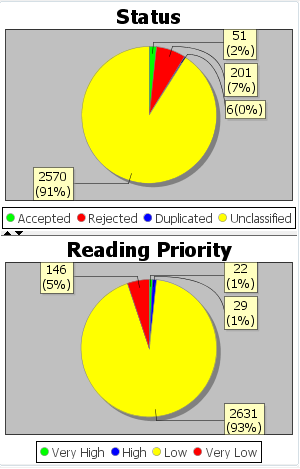
\includegraphics[width = 10cm, height=15cm]{img/extra__oRSLStArt.png}
\caption{Amostragem da extração de Artigos na ferramenta StArt.}
\label{fig:StArt}
\end{figure}



%%%%%%%%%%%%%%%%%%%%%%%%%%%%%%%%%%%%%%%%%%%%%%%%%%%%%%%%%%%%%%%%%%%%%%%%%%%%%%%%
%%%%%%%%%%%%%%%%%%%%%%%%%%%%%%%%%%%%%%%%%%%%%%%%%%%%%%%%%%%%%%%%%%%%%%%%%%%%%%%%
%%%%%%%%%%%%%%%%%%%%%%%%%%%%%%%%%%%%%%%%%%%%%%%%%%%%%%%%%%%%%%%%%%%%%%%%%%%%%%%%
\section{Estado da Arte}
Após a realização da pesquisa dos trabalhos nas bases digitais e a seleção dos trabalhos para a leitura com base no objetivo e questões da proposta obteve-se a fundamentação dos seguintes itens:
\begin{itemize}
\item Monitoramento de sistemas distribuídos
\item Web services
\item Agentes de monitoramento
\item Protocolo SNMP
\item Armazenamento das Informações monitoradas
\item Desempenho
\end{itemize}

\subsubsection{Monitoramento de sistemas distribuídos}
Na realização da pesquisa nos trabalhos selecionados percebeu-se a necessidade do monitoramento de sistemas distribuídos, devido a grande quantidade de  aplicações, dispositivos e web services em funcionamento, e que normalmente não possuem acompanhamento durante o funcionamento. Em \cite{cirstoiu2007monitoring} descrito sobre o monitoramento de sistemas distribuídos e da utilização das API's para a comunicação de aplicativos e a preocupação com o baixo acoplamento dessas ferramentas. Em outro trabalho \cite{joyce1987monitoring} é descrito sobre a importância do monitoramento de sistemas distribuídos, e a utilização testes de programas de para a verificação dos sistemas monitorado. No entanto em \cite{abdu1996monitoring} é descrito o quanto é complexo o gerenciamento do monitoramento de sistemas distribuídos, sendo necessário a utilização de técnicas e métricas para obtenção dos resultados coletados, por conta da grande quantidade de informações geradas pelo monitoramento.  

\subsubsection{Web services}

Os trabalhos \cite{patil2012remote,casola2009sensim} apresentam como a flexibilidade e agilidade no desenvolvimento de \textit{web services}, podem trazer resultados imediatos para as aplicações, suas características que facilitam a integração dos serviços e sistemas e como é fácil a integração de ambientes com os padrões da Indústria e protocolos como SOAP, HTTP e etc., porém a facilidade abre uma preocupação referente a segurança das aplicações, principalmente no que tange a integridade e confidencialidade dos dados, uma dessas ameaças é o \textit{SQL Injection}. 

\subsubsection{Agentes de monitoramento}

Agentes de monitoramento podem ser um dispositivo ou um software, esses podem ser utilizados para realizar a comunicação ou notificação do monitoramento de outros dispositivos ou sistemas distribuídos. Em \cite{smith2008flexible} é descrito sobre a utilização e comparação de ferramentas(\textit{plugins}) que funcionam como agentes de monitoramento de sistemas distribuídos e também da arquitetura definida para o gerenciamento e acompanhamento. No trabalho \cite{puatruct2010agent} é descrito sobre o experimento com informações metacognitivas que proporcionaram 12 definições para a identificação de agentes inteligentes, propostas para a definição de um agente ou Super agente, e como eles podem monitorar sistemas para realização de comunicação homem-máquina.

\subsubsection{Protocolo SNMP}

Em \cite{deGeus} é descrita a definição de um modelo computacional configurável para o gerenciamento e monitoramento de redes, servidores, armazenamento, aplicações e serviços com a utilização do protocolo SNMP para realização de coleta de informações para que sejam criadas métricas onde se possa obter resultados satisfatórios dos serviços disponibilizados. No  trabalho \cite{daSilva} são explicadas informações do protocolo SNMP, como o seu funcionamento, sua utilização , Agente(processo), os tipos de Agente, o Gerente que é uma aplicação, em execução em uma estação de gerenciamento, as operações do protocolo, como por exemplo, \textit{GetRequest, 	GetNextRequest,  GetResponse,  SetRequest  e Trap} e também sobre as ferramentas de monitoramento que são compatíveis com o protocolo, inclusive em \cite{Fraga} é destacado que o protocolo SNMP tem sido o principal protocolo utilizado para gestão e monitoramento de redes. Entretanto, em \cite{deMello} são descritos e identificados alguns pontos fracos do protocolo \acrshort{SNMP}. Apesar  de  seu  nome,  \textit{"Simple  Network  Management  Protocol"},  o  SNMP  é  um protocolo  relativamente  complexo  para  implementar.  Também,  o  SNMP  não  é  um protocolo muito eficiente. Nos trabalhos \cite{phan2009cryptanalysis,subramanyan2000scalable} também são relatados alguns pontos fracos como a vulnerabilidade presente no SNMPv1 , desempenho e falta de escalabilidade.

\subsubsection{Armazenamento das Informações monitoradas}

O Monitoramento dos sistemas distribuídos quando implementados geram informações durante a execução, essas informações são importantes para acompanhar o funcionamento de sistemas distribuído e \textit{web services}. No trabalho \cite{phan2009cryptanalysis} é descrito sobre a importância da coleta dessas informações e a coleta em larga escala utilizando instruções e comandos SQL. Porém devido ao grande número de sistemas distribuídos monitorados e a grande quantidade de informações geradas por meio do monitoramento, nos trabalhos \cite{abdu1996monitoring,hirate2009profiling} são apresentadas as técnicas para mensurar a sobrecarga gerada pela quantidade de informações e padrões de mineração dos dados armazenados.  

\subsubsection{Desempenho}

O trabalho \cite{wang2016improvements} apresenta algoritmos de compactação de dados, para a realização de transferência dos dados de modo otimizado, devido a grande quantidade de informações geradas durante o monitoramento dos sistemas distribuídos. Nesse trabalho foram realizados vários testes, incluído conversão de formatos, como por exemplo, arquivos XML. Em \cite{kotsopoulos2008soa} é descrito o motivo da não utilização do protocolo SNMP, por conta de algumas limitações, como por exemplo, a escalabilidade e eficiência. 


%%%%%%%%%%%%%%%%%%%%%%%%%%%%%%%%%%%%%%%%%%%%%%%%%%%%%%%%%%%%%%%%%%%%%%%%%%%%%%%%
%%%%%%%%%%%%%%%%%%%%%%%%%%%%%%%%%%%%%%%%%%%%%%%%%%%%%%%%%%%%%%%%%%%%%%%%%%%%%%%%
%%%%%%%%%%%%%%%%%%%%%%%%%%%%%%%%%%%%%%%%%%%%%%%%%%%%%%%%%%%%%%%%%%%%%%%%%%%%%%%%